%
% This is a borrowed LaTeX template file for lecture notes for CS267,
% Applications of Parallel Computing, UCBerkeley EECS Department.
% Now being used for CMU's 10725 Fall 2012 Optimization course
% taught by Geoff Gordon and Ryan Tibshirani.  When preparing 
% LaTeX notes for this class, please use this template.
%
% To familiarize yourself with this template, the body contains
% some examples of its use.  Look them over.  Then you can
% run LaTeX on this file.  After you have LaTeXed this file then
% you can look over the result either by printing it out with
% dvips or using xdvi. "pdflatex template.tex" should also work.
%

\documentclass[twoside]{article}
\setlength{\oddsidemargin}{0.25 in}
\setlength{\evensidemargin}{-0.25 in}
\setlength{\topmargin}{-0.6 in}
\setlength{\textwidth}{6.5 in}
\setlength{\textheight}{8.5 in}
\setlength{\headsep}{0.75 in}
\setlength{\parindent}{0 in}
\setlength{\parskip}{0.1 in}

%
% ADD PACKAGES here:
%

\usepackage{amsmath,amsfonts,graphicx}
\usepackage[siunitx]{circuitikz}


%
% The following commands set up the lecnum (lecture number)
% counter and make various numbering schemes work relative
% to the lecture number.
%
\newcounter{lecnum}
\renewcommand{\thepage}{\thelecnum-\arabic{page}}
\renewcommand{\thesection}{\thelecnum.\arabic{section}}
\renewcommand{\theequation}{\thelecnum.\arabic{equation}}
\renewcommand{\thefigure}{\thelecnum.\arabic{figure}}
\renewcommand{\thetable}{\thelecnum.\arabic{table}}

%
% The following macro is used to generate the header.
%
\newcommand{\lecture}[4]{
   \pagestyle{myheadings}
   \thispagestyle{plain}
   \newpage
   \setcounter{lecnum}{#1}
   \setcounter{page}{1}
   \noindent
   \begin{center}
   \framebox{
      \vbox{\vspace{2mm}
    \hbox to 6.28in { {\bf EEE 202: Circuits I
	\hfill Fall 2018} }
       \vspace{4mm}
       \hbox to 6.28in { {\Large \hfill Lecture #1: #2  \hfill} }
       \vspace{2mm}
       \hbox to 6.28in { {\it Lecturer: #3 \hfill Scribe: #4} }
      \vspace{2mm}}
   }
   \end{center}
   \markboth{Lecture #1: #2}{Lecture #1: #2}

   \vspace*{4mm}
}
%
% Convention for citations is authors' initials followed by the year.
% For example, to cite a paper by Leighton and Maggs you would type
% \cite{LM89}, and to cite a paper by Strassen you would type \cite{S69}.
% (To avoid bibliography problems, for now we redefine the \cite command.)
% Also commands that create a suitable format for the reference list.
\renewcommand{\cite}[1]{[#1]}
\def\beginrefs{\begin{list}%
        {[\arabic{equation}]}{\usecounter{equation}
         \setlength{\leftmargin}{2.0truecm}\setlength{\labelsep}{0.4truecm}%
         \setlength{\labelwidth}{1.6truecm}}}
\def\endrefs{\end{list}}
\def\bibentry#1{\item[\hbox{[#1]}]}

%Use this command for a figure; it puts a figure in wherever you want it.
%usage: \fig{NUMBER}{SPACE-IN-INCHES}{CAPTION}
\newcommand{\fig}[3]{
			\vspace{#2}
			\begin{center}
			Figure \thelecnum.#1:~#3
			\end{center}
	}
% Use these for theorems, lemmas, proofs, etc.
\newtheorem{theorem}{Theorem}[lecnum]
\newtheorem{lemma}[theorem]{Lemma}
\newtheorem{proposition}[theorem]{Proposition}
\newtheorem{claim}[theorem]{Claim}
\newtheorem{corollary}[theorem]{Corollary}
\newtheorem{definition}[theorem]{Definition}
\newenvironment{proof}{{\bf Proof:}}{\hfill\rule{2mm}{2mm}}

% **** IF YOU WANT TO DEFINE ADDITIONAL MACROS FOR YOURSELF, PUT THEM HERE:

\newcommand\E{\mathbb{E}}

\begin{document}
%FILL IN THE RIGHT INFO.
%\lecture{**LECTURE-NUMBER**}{**DATE**}{**LECTURER**}{**SCRIBE**}
\lecture{2}{Circuit Elements and Ohms Law}{Bahman Moraffah}{Ryan Jones}
%\footnotetext{These notes are partially based on those of Nigel Mansell.}

% **** YOUR NOTES GO HERE:

% Some general latex examples and examples making use of the
% macros follow.  
%**** IN GENERAL, BE BRIEF. LONG SCRIBE NOTES, NO MATTER HOW WELL WRITTEN,
%**** ARE NEVER READ BY ANYBODY.
\section{Things to remember}
\begin{itemize}
	\item $I = \frac{dq}{dt}$
	\item $P = \frac{dw}{dt}$
	\item $P = \frac{dw}{dt} = \frac{dw}{dq} * \frac{dq}{dt} = VI$ 
\end{itemize}

\begin{figure}[h!]
\begin{center}
\begin{circuitikz}[american]
\draw (0,0) to[V=10V,invert, i_=$i_1$] (2,0);
\end{circuitikz}
\caption{Power is absorbing if current is going from + to -}
\end{center}
\end{figure}

\begin{figure}[h!]
\begin{center}
\begin{circuitikz}[american]
\draw (0,0) to[V=10V, i_=$i_1$] (2,0);
\end{circuitikz}
\caption{Power is supplying if current is going from - to +}
\end{center}
\end{figure}




\newpage
\section{Elements in a Circuit}
In order to build a circuit we need a bunch of elements.
Elements in a circuit are either Passive or Active

\begin{itemize}
\item Passive Elements:
  Elements that cannot generate energy (e.g., Resistor, Capacitor, Inductor)
\item Active Elements:
  Elements that can actually generate energy (e.g., Voltage/Current Source)
\end{itemize}

\subsection{Types of Sources}
\begin{itemize}
\item Independent Sources: Value does not depend on any other element in a circuit.

\begin{circuitikz}[american currents]
\draw (0,0) to [I=$Current Source$] (0,2);
\end{circuitikz}

\begin{circuitikz}[american voltages]
\draw (0,0) to[V=$Voltage Source$] (0,2);
\end{circuitikz}


\item Dependent Sources: The value of that source is controlled by another source.
  \newline
  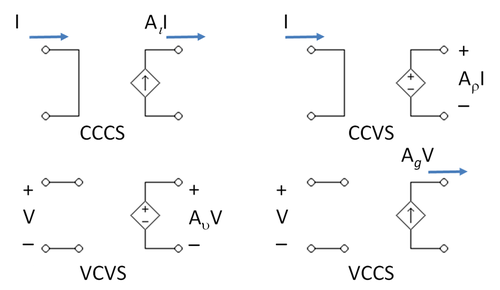
\includegraphics[scale=0.70]{dependentsources}
  \begin{enumerate}
  \item Voltage Sources that are controlled by a voltage (VCVS)
  \item Voltage Sources that are controlled by current (VCCS)
  \item Current Source controlled by a voltage (CCVS)
  \item Current Source controlled by current (CCCS)
  \end{enumerate}
\end{itemize}

\newpage
\section{Ohm's Law (V = IR)}
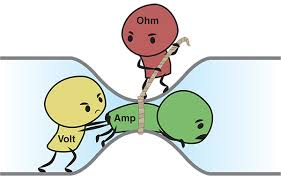
\includegraphics[scale=0.75]{ohm}
\begin{itemize}
	\item Resistance ($\Omega$): Opposition to the flow of charge. 
	\item Resistor: Element that impedes or doesn't let element go
	\newline
	\begin{circuitikz}
	\draw (0,0) to[R, l=$R_1$] (2,0);
	\end{circuitikz}

	\item Conductance ($S$): Inverse of Resistance 
		\begin{enumerate}
			\item $G = \frac{1}{R}$ 
			\item Measured in siemens 
		\end{enumerate}
	
	\item Relationship between Voltage, Resistance, and Current is through Ohm's Law
	
	\begin{enumerate}
		\item $I \propto V$
		\item $I \propto \frac{1}{R}$
		\item $I = \frac{V}{R}$
		\item $P = VI$
	\end{enumerate}

	\item You can find the unknown by knowing 2 of the Ohm's law variables. This also allows us to substitute Ohm's Law into more formulas. 

	\begin{enumerate}
		\item $V = RI \Rightarrow  P = (RI)I = RI^2 > 0$ 
		\item $I = \frac{V}{R} \Rightarrow  P = V * \frac{V}{R} = \frac{V^2}{R} > 0$\item These two functions are always positive which tells us if we have resistance in a circuit it's always absorbing power not supplying it. 
	\end{enumerate}
	
	\newpage
	\section{Kirchhoff Law}
	\item Node: The portion of a wire that makes up a bunch of elements
	\item Kirchhoff Current Law: Sum of the current entering the node is equal to the sum of the currents that are leaving. In other words, Algebraic sum of the currents adds up to zero with the following rule:
	\begin{itemize}
	\item If Current enters a node $\rightarrow$ $(+) $
	\item If Current leaves a node $\rightarrow$ $(-) $
	\end{itemize}
	\hspace{3cm}Then $\Sigma I = 0$
	\newline
	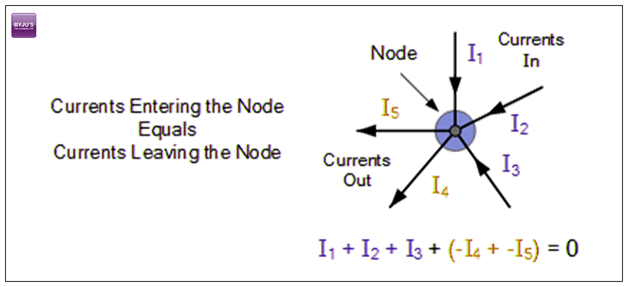
\includegraphics[scale=0.75]{currentlaw}
	\item Kirchoff Voltage Law: Within any closed loop of a circuit, the sum of all the voltages in any closed loop is always zero with the following rule:
	\begin{itemize}
	\item Voltage encounters $+$ $\rightarrow$ $(+) $
	\item Voltage encounters $-$ $\rightarrow$ $(-) $
	\end{itemize}
	\hspace{3cm}Then $\Sigma V = 0$
	%\newline
	
	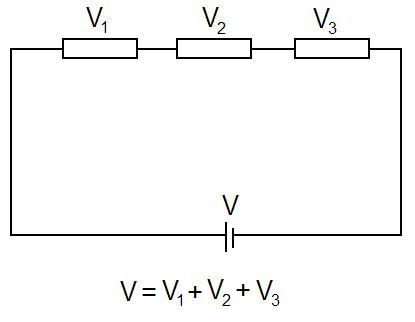
\includegraphics[scale=0.70]{voltagelaw}

	\subsection{Example 1}
	\begin{circuitikz} \draw
	(0,0) to[american voltage source, l=36 <\volt>, invert] (0,4)
		  to [short, i=$$] (1,4) 
		  to[generic, l=$+ 12V -$] (4,4)
		  to[generic, l=$+ 8V -$] (8,4)	
		  to[generic, l=$+ 16V -$] (8,0)
		  
	(0,0) to [short] (8,0)
	(4,0) to[american controlled voltage source, *-*, l=24<\volt>, i=$I_x$] (4, 4)
		 
	%(0.5,0) -- (0.5, -2)
	%	   to[voltmeter, l=3<\kilo\volt>, color=blue] (3.5,-2) -- (3.5,0)
 	;
 	\end{circuitikz}

\end{itemize}

\begin{itemize}
\item Power Supplied = Power Absorbed
\item P = VI
\item $P_{36}$ is supplying power
\item $P_{36} = -36*I_x (absorbing)$
\item $P_1 = 12I_x (absorbing)$
\item $P_2 = 8I_x (absorbing)$
\item $P_3 = 16I_x (absorbing)$
\item $P_{2I} = 24*2I_{x} = 48I_{x} (absorbing)$

\end{itemize}




% **** THIS ENDS THE EXAMPLES. DON'T DELETE THE FOLLOWING LINE:

\end{document}





